\documentclass[11pt]{article}
%\usepackage[spanish]{babel} 
%\selectlanguage{english}  
\usepackage[utf8]{inputenc} 
\usepackage[T1]{fontenc} 
\usepackage{array}
\usepackage{geometry}
 \geometry{
 a4paper,
 total={170mm,257mm},
 left=20mm,
 top=20mm,
 }
\usepackage{amsmath, amsthm, amsfonts} 
\usepackage{graphicx} 
\usepackage[colorinlistoftodos]{todonotes} 
\usepackage[colorlinks=true, allcolors=blue]{hyperref} 
\usepackage[square,numbers]{natbib}
\usepackage{upgreek}
\usepackage{lipsum}  
\usepackage{diagbox}


\title{Informe del Proyecto Final Grupo 6}
\author{Benjam\'in Ignacio Ayala Baeza  \\ \href{mailto:beayala2021@udec.cl}{beayala2021@udec.cl} 
        \and Mar\'ia Ignacia Espinoza Inzunza \\ \href{mailto:marespinoza2021@udec.cl}{marespinoza2021@udec.cl} \\
        \and Florencia Andrea Fuentes Jara \\ \href{mailto:flofuentes2021@udec.cl}{flofuentes2021@udec.cl} \\
        \and Mart\'in Andrés Sepúlveda Zu\~niga \\ \href{mailto:msepulveda2021@udec.cl}{msepulveda2021@udec.cl} \\
\date{Universidad de Concepci\'on \\ \today}
}
\setlength{\marginparwidth}{2cm}

%-------------------------------------------------------------------------------------------------------------------------

\begin{document}

\maketitle

\begin{abstract}
En el presente documento buscamos encontrar la relación entre la distancia de lanzamiento de una fuerza aplicada a un cuerpo circular y el giro que se produce. Esto midiendo el número de giros a distintas distancias del cuerpo y con varias repeticiones para eliminar el error aleatorio. Además graficamos nuestros datos y realizamos varios ajustes para analizar cuál se asimila más a nuestro modelo esto viéndolo con el análisis de sus respectivos residuos y así concluir con alguna correspondencia entre nuestras variables.
\end{abstract}

\section{Introducción} \label{intro}
 En este informe decidimos realizar un proyecto que surgió bajo el interés de saber cuanto rota una cinta métrica al lanzar la espiga a distintas distancias de la cinta, en términos físicos, nuestra premisa para este experimento consta de estudiar de una manera eficaz los efectos de una fuerza aplicada de manera tangencial a un objeto que posee una capacidad de rotación.
 \medskip
 Primero, definiremos algunos conocimientos previos necesarios para poder eventualmente comparar el comportamiento de los datos con los fenómenos físicos, luego ilustraremos los procedimientos necesarios que realizaremos en la etapa de experimentación, además de los resultados obtenidos en esta y poder así realizar ajustes con distintos modelos con el fin de analizar si estos se asimilan a el comportamiento natural de estos datos a través del análisis de sus residuos. Finalmente concluiremos explicando cual modelo se ajusta mejor a los datos y como este comportamiento corresponde a lo esperado por las leyes de la física. 

\section{Objetivos}
Nuestros objetivos a lograr con esta actividad de laboratorio son :

\begin{itemize}
    \item Encontrar la relación entre la distancia de lanzamiento del medidor de una cinta métrica con el número de giros que esta hace en una plataforma en nuestro caso la mesa del laboratorio.
    \item Comparar nuestros resultados con algún hecho cotidiano o fenómeno físico relacionado.
\end{itemize}

\section{Marco Teórico}
Para el desarrollo de este informe haremos uso de las siguientes ecuaciones y términos físicos:

\begin{itemize}
   
    \item \textbf{Ángulo de rotación:} Medida del giro de una figura alrededor de un punto fijo.\cite{angulo}
    
    \item \textbf{Fuerza:} Acción, esfuerzo o influencia que puede alterar el estado de movimiento o de reposo de cualquier cuerpo. El cual se puede medir con la siguiente formula dada por la segunda ley de newton \cite{fundamentos} :
        
        \begin{equation}
           \vec{F} = m \vec{a}
           \label{eq:fuerza}
        \end{equation} 
    
    \item \textbf{Aceleración Tangencial:} Magnitud vectorial que permite expresar el aumento de velocidad en una unidad de tiempo relacionado a un movimiento circular.
    
    \item \textbf{Fuerza Tangencial:} Fuerza que actúa sobre un cuerpo en un movimiento circular en la dirección tangencial de una trayectoria curva.

\end{itemize}

\section{Experimentación}
Para encontrar la correlación entre distancia y cantidad de vueltas del cuerpo de la cinta de medir, debemos repetir el experimento en diversas condiciones. Nuestra condición variable corresponde a la distancia desde la cual veremos como afecta la fuerza de choque tangencial de la espiga con el cuerpo de esta.

\subsection{Materiales}
En este proyecto utilizamos los siguientes instrumentos:
\begin{itemize}
    \item[-] Cinta Métrica 3$[\text{m}]$
    \item[-] Papel con ejes de referencia
    \item[-] Cinta adhesiva
    \item[-] Celular con cámara lenta
    \item[-] Mesa
\end{itemize}
    
\subsection{Montaje Experimental}
  En la figura \ref{fig:montaje} mostramos los materiales utilizados para el montaje de nuestro experimento.
  
\begin{figure}[ht]
    \centering
    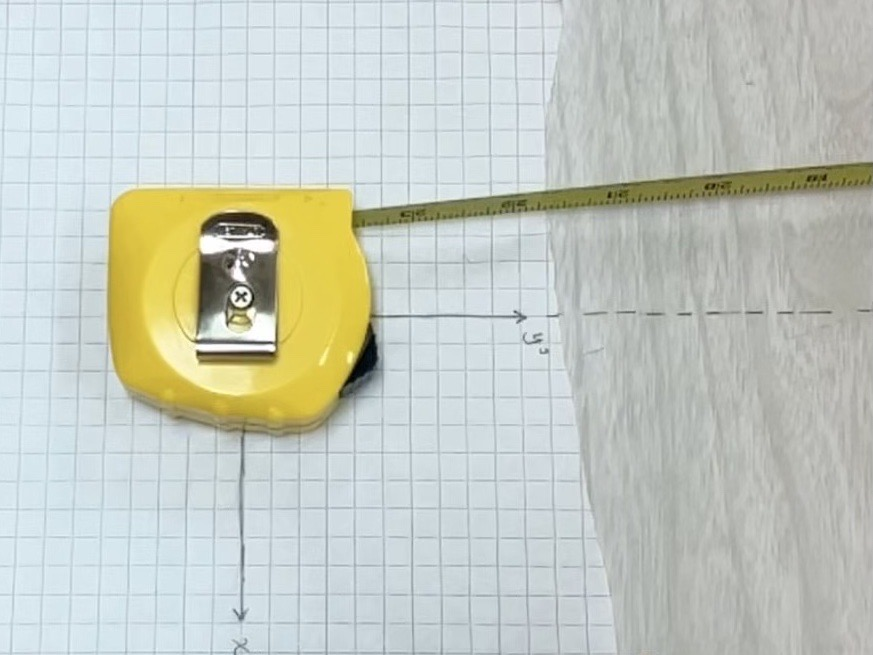
\includegraphics[scale=0.25]{Informe/img/montaje1.png}
    \caption{Fotografía de montaje experimental}
    \label{fig:montaje}
\end{figure}
    
\subsection{Procedimiento}
A continuación describiremos detalladamente el paso a paso realizado para las diversas mediciones hechas:

\begin{enumerate}
    \item Comenzamos colocando la cinta métrica al centro del papel con ejes de referencia, de forma que si extendemos la cinta métrica esta crece a lo largo del eje de las ordenadas. La cinta métrica y debe estar pegada al papel, esto lo logramos usando la cinta adhesiva.
    \item Alineamos en nuestra mesa el papel con ejes de referencia y proyectamos estos ejes en la mesa, de forma que tengamos una extensión de estos para observar cuanto gira el montaje de la cinta métrica con el papel. 
    \item Posicionamos nuestro celular con cámara lenta por encima del montaje del papel, mesa y cinta de forma que tengamos una visión área del sistema.
    \item Tomamos la espiga de la cinta métrica y la extendemos hasta llegar a los $10[\text{cm}]$, luego soltamos esta y vemos cuanto giro se produce. Todo este proceso se graba con el celular. \label{4} 
    \item Repetimos el paso \ref{4} diez veces. \footnote{Idealmente recomendamos tomar más repeticiones, ya que entre más repeticiones menos error aleatorio va a existir, sin embargo, para este proyecto en particular por temas de tiempo tuvimos que mantenernos en diez repeticiones.}
    \item Repetimos todo el procedimiento para la medida de la cinta métrica en incrementos de $10[\text{cm}]$, hasta llegar a los $100[\text{cm}]$.
\end{enumerate}

\subsection{Procesamiento de datos}
El procedimiento para la extracción de datos, en este caso el ángulo total de giro, se hizo mediante el análisis de imágenes que se extrajeron de los vídeos, considerando este ángulo de giro desde que la espiga de la cinta métrica choca con el cuerpo de esta, y hasta que este deja de girar. Para esto se utilizo un programa de edición de imágenes con el que contaba con una escuadra digital, la cual tenia una sensibilidad de $0.5^{\circ}$. 

\medskip
Se implementaron dos marcos de referencia en la imagen obtenida, uno se ubico en la superficie en la que se hizo el experimento, la cual se encontraba en reposo, y el segundo se ubico en la cinta métrica, la cual era un sistema dinámico. Luego se comparo el ángulo entre los estados iniciales de cada sistema y el estado final de cada sistema, así obteniendo el ángulo total de giro de la cinta, esto se repitió para cada iteración de longitud.

\section{Resultados y Análisis}
A continuación, expondremos nuestros datos recopilados durante las mediciones, el archivo que contiene estos datos se encuentra en \href{https://github.com/ayalin7/El-proyectito/blob/main/graficos/datos/giro.txt}{este link}, donde cada columna representa los ángulos medidos en cada repetición según la longitud dada. Primero, graficaremos estos datos en la figura \ref{fig:datos}, la cual nos muestra la cantidad de vueltas expuestas según la distancia tomada, donde el eje de las abscisas corresponde a la longitud desde la cual soltamos la espiga de la cinta métrica y el eje ordenado la cantidad de grados que el cuerpo de este ha rotado. \\

Tomando lo visto en la figura \ref{fig:datos} podemos ver la notoria tendencia hacia el incremento de numero de giros cada vez que aumentamos la distancia desde la cual soltamos la espiga de la cinta métrica. A partir de este gráfico, comenzamos un trabajo analítico de los datos recopilados, en el cual realizamos tres ajustes de curvas para poder asociar una función a la tendencia de crecimiento de nuestros datos. 

\medskip

La figura \ref{fig:axb} nos muestra el primer ajuste que realizamos a partir de una función exponencial y la gráfica del residuo generado a partir de dicho ajuste. Al momento de calcular el $\chi^2$ obtenemos un valor de 24.4, el código que utilizamos para generar este gráfico se encuentra en \href{https://github.com/ayalin7/El-proyectito/blob/main/graficos/grafico-modelo-axb.py}{este link}.

\medskip

Continuando con los diversos ajustes realizados, en la figura \ref{fig:asinb} utilizamos una función que tiene asociada una función seno, la cual nos hacer creer a partir de un análisis visual de estar cercano a que la curva recorra todos los puntos expuestos por nuestros datos, lamentablemente, el efecto oscilatorio de la función seno provoca que el valor del $\chi^2$ crezca, haciéndose $\chi^2 = 43.9$ lo cual nos indica de que no estamos frente a un buen ajuste, considerando que el ajuste realizado con la función exponencial nos arrojo un valor mucho mas bajo para el $\chi^2$. \\ El código que utilizamos para generar este ajuste se puede encontrar en \href{https://github.com/ayalin7/El-proyectito/blob/main/graficos/grafico-modelo-asinb.py}{este link}.

\medskip

Finalmente, realizamos el ajuste mostrado en la figura \ref{} basado en una curva que utiliza una función polinomial de grado dos. El código con el cual graficamos y calculamos el $\chi^2$ se puede encontrar en \href{}. Podemos apreciar visualmente la similitud con el gráfico mostrado en la figura \ref{}, sin embargo, al momento de comparar los valores del $\chi^2$ vemos una disminución para este ultimo ajuste en el cual utilizamos la función cuadrática, indicándonos que de los tres ajustes que realizamos, este es el mejor. Hacemos notar que, 

% agregar lo de los diferentes ajutes y como hay una que tiene la mejor curva, en función del chi cuadrado que aumenta en consideración con los diversos coeficientes de las funciones del ajuste. \ref{tabla}

%SACA DEL HOYO DE LA FLO : el martin lo explica



\begin{table}[ht]
\centering
\begin{tabular}{|c|c|c|}
\hline
\small{Longitud del tiro} & Promedio[$\bar{x}$]  & Desviación Estándar [$\sigma$]\\ \hline
 10  \scriptsize{$[\text{cm}]$} & $63.6^\circ$  & $\pm 18.5^\circ$  \\ \hline
 20  \scriptsize{$[\text{cm}]$} & $193.8^\circ$ & $\pm 14.6^\circ$  \\ \hline
 30  \scriptsize{$[\text{cm}]$} & $266.1^\circ$ & $\pm 34.2^\circ$  \\ \hline
 40  \scriptsize{$[\text{cm}]$} & $370.8^\circ$ & $\pm 81.8^\circ$  \\ \hline
 50  \scriptsize{$[\text{cm}]$} & $439.3^\circ$ & $\pm 89.0^\circ$  \\ \hline
 60  \scriptsize{$[\text{cm}]$} & $495.5^\circ$ & $\pm 79.9^\circ$  \\ \hline
 70  \scriptsize{$[\text{cm}]$} & $508.9^\circ$ & $\pm 76.5^\circ$  \\ \hline
 80  \scriptsize{$[\text{cm}]$} & $621.3^\circ$ & $\pm 97.8^\circ$  \\ \hline
 90  \scriptsize{$[\text{cm}]$} & $621.6^\circ$ & $\pm 97.4^\circ$  \\ \hline
 100 \scriptsize{$[\text{cm}]$} & $682.8^\circ$ & $\pm 75.5^\circ$  \\ \hline 
\end{tabular}
\caption{Promedio y desviación estándar de las iteraciones mediadas en cada longitud de tiro}
\label{tabla}
\end{table}

\begin{figure}[ht]
    \centering
    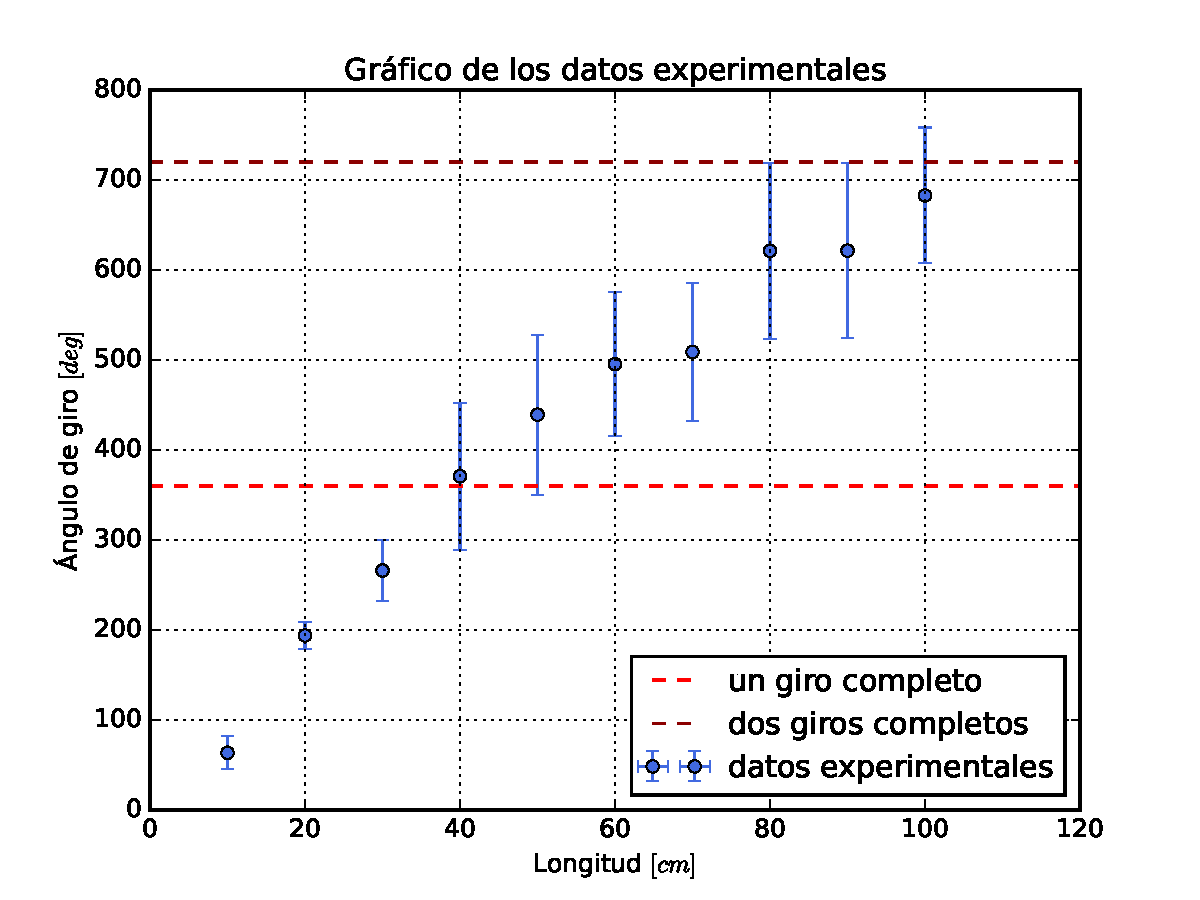
\includegraphics[scale=0.5]{Informe/img/grafico-datos.pdf}
    \caption{Gráfico formado a partir de los datos recopilados.}
    \label{fig:datos}
\end{figure}

\begin{figure}[ht]
    \centering
    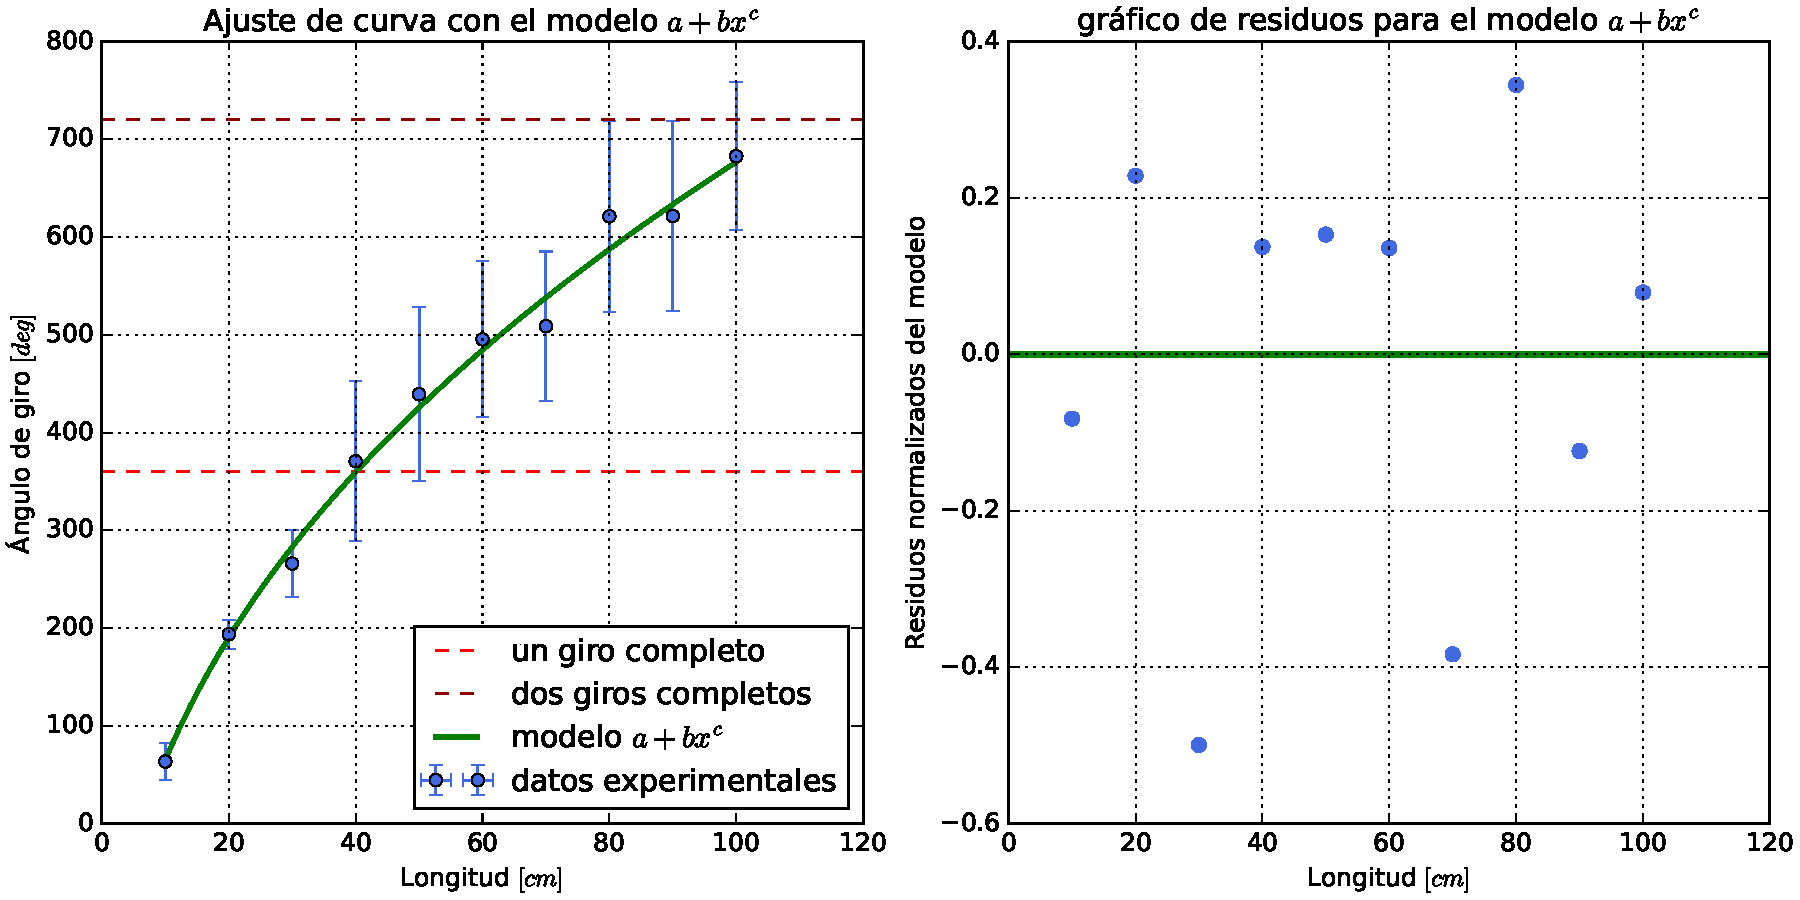
\includegraphics[scale=0.5]{Informe/img/grafico-modelo-axb.pdf}
    \caption{Gráfico del modelo $a + bx^{c}$, con su respectivo análisis de residuos, donde $\chi^2 = 24.4$.}
    \label{fig:axb}
\end{figure}

\begin{figure}[ht]
    \centering
    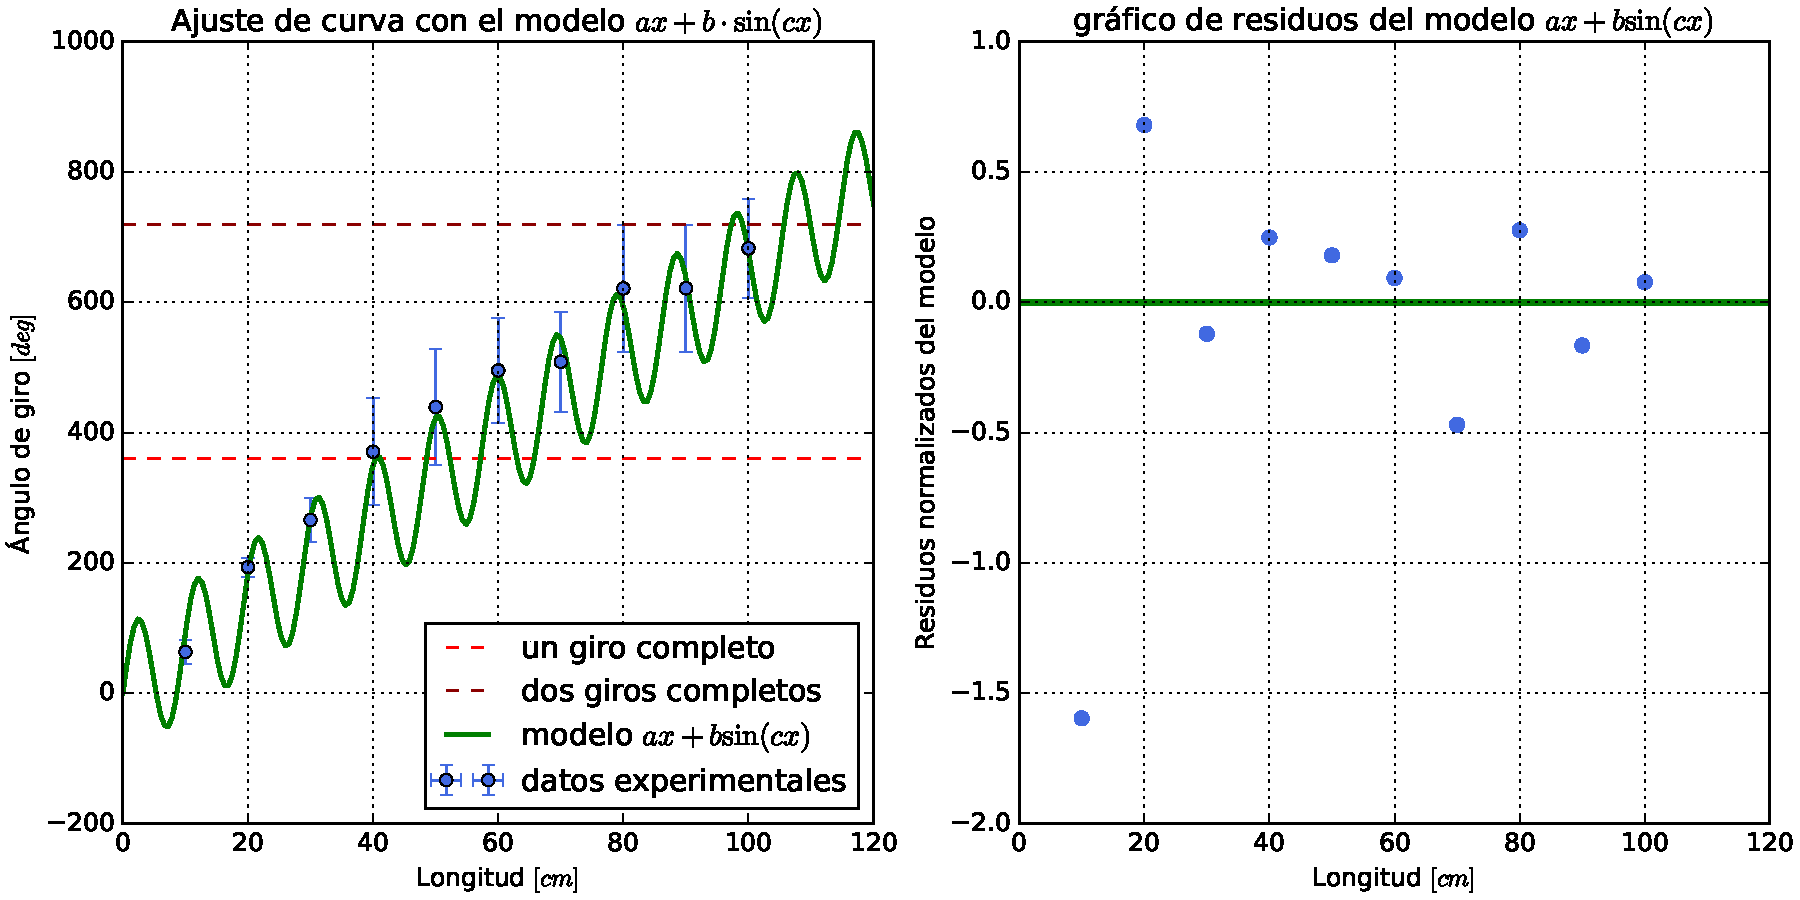
\includegraphics[scale=0.5]{Informe/img/grafico-modelo-asinb.pdf}
    \caption{Gráfico del modelo $ax + b\sin(cx)$, con su respectivo análisis de residuos, donde $\chi^2 = 43.9$.}
    \label{fig:asinb}
\end{figure}

\begin{figure}[ht]
    \centering
    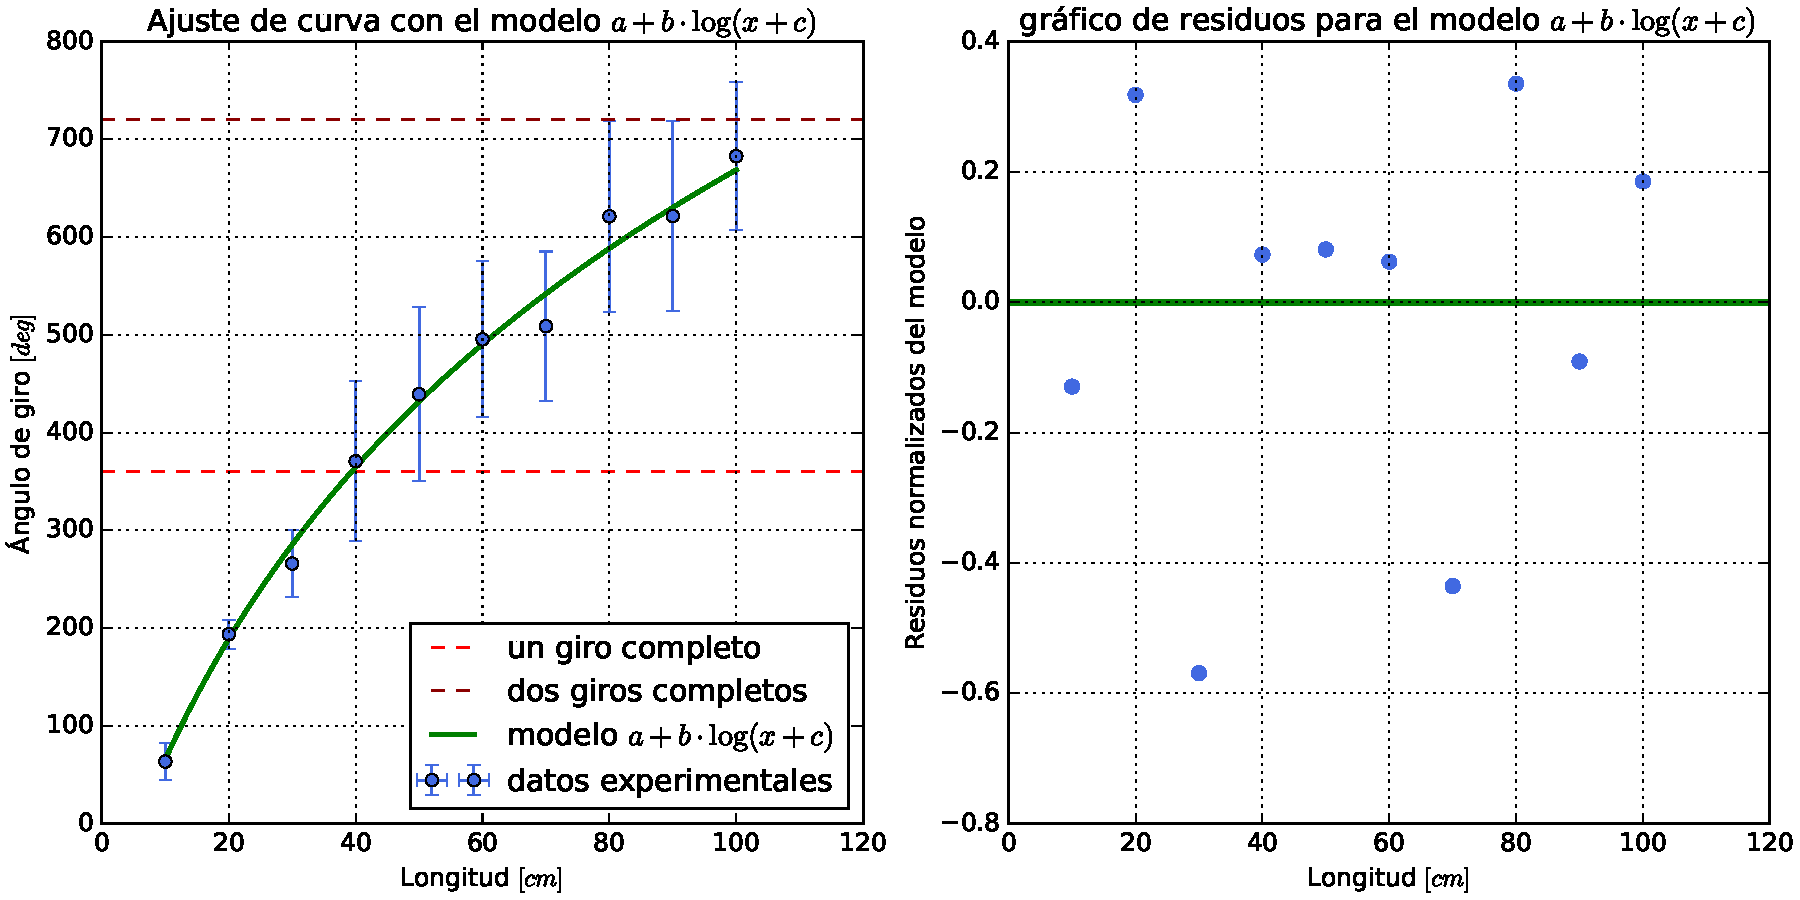
\includegraphics[scale=0.5]{Informe/img/grafico-modelo-alogb.pdf}
    \caption{Gráfico del modelo $a + b \cdot \log(x + c)$, con su respectivo análisis de residuos, $\chi^2 = 21.1$.}
    \label{fig:alogb}
\end{figure}

\section{Conclusión}
Como visto anteriormente en el análisis, los resultados a través de las tablas y los gráficos podemos concluir que el modelo que más se ajusta a la gráfica de los datos \ref{fig:datos} y la función $a + bx + cx^2$ donde a es nuestro coeficiente de 

%Se concluye lo concluido por la conclusión que queda concluido lo que concluye finalmente.

\pagebreak

\bibliographystyle{apalike}
\bibliography{Informe/referencias.bib}

\end{document}